%-----------------------------------------------------------------------------%
\chapter{LANDASAN TEORI}
%-----------------------------------------------------------------------------%
Bab ini menjelaskan teori-teori yang berkaitan mengenai teori penunjang dan jurnal terkait yang digunakan dalam proses penelitian tugas akhir ini. \\

%
\vspace{4.5pt}

\section{Tinjauan Pustaka}
\noindent Penelitian ini menggunakan beberapa teori terkait yang diperlukan dalam pengerjaan yang dilakukan. Penjelasan mengenai teori-teori tersebut akan dijelaskan sebagai berikut. \\

\subsection{Citra Digital}
\label{subsec:CitraDigital}
\noindent Citra digital merupakan sebuah fungsi dua dimensi \textit{f(x,y)}, di mana \textit{x} dan \textit{y} adalah koordinat, dan nilai \textit{f} menyatakan intensitas atau tingkat keabuan yang dimiliki citra pada titik atau \textit{pixel} (\textit{picture element}) tersebut. Nilai \textit{f} merupakan nilai berhingga dan bersifat diskrit \cite{gonzalez}.\\
\noindent Jenis citra digital bergantung pada jenis perangkat keras yang digunakan dan dapat dikelompokkan ke dalam beberapa jenis model warna, yang paling umum digunakan adalah model RGB. Citra model RGB merupakan citra yang menggunakan 3 kombinasi warna, yaitu merah, hijau, dan biru. Pada citra RGB 24-bit, setiap warna mempunyai nilai \textit{f} antara 0 hingga 255 sehingga perpaduan dari ketiga warna tersebut akan menghasilkan $256^{3}$ jenis warna \cite{gonzalez}. \\

\subsection{Pengolahan Citra}
\noindent Pengolahan citra dapat didefinisikan sebagai suatu bidang yang menggunakan citra sebagai masukan, lalu masukan tersebut diolah sehingga menghasilkan citra kembali. Berdasarkan definisi tersebut, perhitungan rata-rata dari suatu citra yang menghasilkan sebuah angka tidak termasuk pengolahan citra \cite{gonzalez}.\\
\noindent Terdapat satu paradigma yang mengkategorikan 3 jenis proses komputasi dalam pengolahan citra, yaitu tingkat rendah, tingkat sedang, dan tingkat tinggi. Proses tingkat rendah mencakup operasi yang sangat sederhana seperti \textit{image preprocessing} untuk mengurangi \textit{noise}, meningkatkan kontras, dan mempertajam citra. Proses tingkat sedang meliputi segmentasi untuk membagi daerah citra menjadi \textit{region} atau objek. Sedangkan proses tingkat tinggi memampukan komputer untuk mengerti seperti pengenalan objek dan analisis citra \cite{gonzalez}. \\

\subsection{Pengabuan Citra}
\noindent Citra RGB yaitu citra berwarna memiliki ukuran yang lebih besar dibandingkan dengan citra \textit{grayscale}. Untuk mempercepat proses komputasi pada citra, maka citra RGB perlu diubah menjadi citra \textit{grayscale} dengan skala keabuan 256. Persamaan pengabuan citra dapat dilihat pada persamaan \ref{eq:grayscale} dengan \textit{R} melambangkan intensitas warna merah, \textit{G} untuk intensitas warna hijau, dan \textit{B} untuk intensitas warna biru. 

\begin{table}[H]
	\begin{adjustbox}{width=1\textwidth}
		\begin{tabular}{|p{13.55cm}|}
			\hline
			\begin{equation}
			Gray value = 0.299 R + 0.587 G + 0.114 B
			\label{eq:grayscale}
			\end{equation}\\
			\hline
		\end{tabular}
	\end{adjustbox}
\end{table}

\noindent Persamaan \ref{eq:grayscale} menyimpulkan bahwa persentase warna hijau yang paling besar karena manusia cenderung lebih sensitif terhadap perubahan warna hijau yang memiliki panjang gelombang sekitar 500-570 nm, merah, lalu biru \cite{ragb}, dan merupakan rekomendasi dari \textit{International Telecommunication Union Radiocommunication Sector}.\\

\subsection{Deteksi Tepi}
\noindent Tepian memiliki arti yaitu terjadinya perubahan intensitas secara signifikan pada sebuah citra. Deteksi tepi yang digunakan pada penelitian ini adalah dengan menggunakan operator \textit{Canny} untuk mendapatkan tepian citra sebesar 1 piksel. Proses deteksi tepi Canny memiliki tahapan sebagai berikut:
\begin{enumerate}
	\item Penghalusan \\
	Pada tahapan pertama citra dihaluskan dengan \textit{Gaussian filter} untuk mengurangi derau yang dapat menghasilkan detail yang mengganggu.
	\item Menghitung Gradien \\
	Untuk menghitung gradien yang dapat menghasilkan tepian yang masih tebal dengan beberapa operator, diantaranya adalah Sobel, Prewitt, atau Robert.
	\item \textit{Non-maxima Supression} \\
	Tahapan ini digunakan untuk menipiskan tepian tebal yang diperoleh dari operasi sebelumnya dengan cara mencari nilai maksimum di tepian.
	\item \textit{Double Thresholding} \\
	Dari hasil \textit{non-maxima supression} bisa ditemukan tepian yang belum sempurna, sehingga perlu dilakukan \textit{thresholding} untuk menghilangkan derau yang tidak diinginkan. Caranya adalah dengan menetapkan 2 nilai \textit{threshold} yaitu \textit{high threshold} dan \textit{low threshold} untuk menentukan apakah piksel tersebut akan masuk dalam \textit{threshold} untuk dijadikan tepian. Piksel yang nilainya berada di atas \textit{high threshold} akan menjadi tepian kuat, sebaliknya jika di bawah \textit{low threshold} akan dijadikan sebagai \textit{background}.
	\item \textit{Edge Tracking} \\
	Tahapan terakhir yaitu \textit{Edge Tracking} atau \textit{Edge Linking} digunakan untuk menghubungkan tepian kuat dan tepian lemah yang nilai pikselnya berada diantara \textit{high threshold} dan \textit{low threshold}. Ketika tepian lemah yang tidak terhubung dengan tepian kuat maka piksel tersebut akan dianggap sebagai \textit{background}. Hasil akhir dari deteksi tepi Canny adalah tepian halus yang memiliki lebar sebesar 1 piksel.\\
\end{enumerate} 

\subsection{\textit{Hough Transform}}
\noindent \textit{Hough Transform} adalah sebuah teknik untuk mengidentifikasi bentuk spesifik dalam sebuah citra. \textit{Hough Transform} mengkonversikan semua titik dalam sebuah kurva ke dalam sebuah lokasi tunggal dalam ruang parametrik (ruang akumulator) lain dengan transformasi koordinat. Metode ini bertujuan untuk memetakan fitur global ke fitur lokal. Konsep ini juga dapat diterapkan untuk mendeteksi garis lurus, lingkaran, elips atau bentuk geometrik lainnya. \textit{Hough Transform} yang digunakan adalah untuk ekstraksi garis lurus. Berikut adalah rumus yang digunakan untuk mencari jarak antara titik \textit{origin} dengan garis yang terbentuk \cite{shih}:

\begin{table}[H]
	\begin{adjustbox}{width=1\textwidth}
		\begin{tabular}{|p{13.55cm}|}
			\hline
			\begin{equation}
			\rho = x\cos(\theta)+y\sin(\theta)
			\label{eq:PersamaanRho}
			\end{equation}\\
			\hline
		\end{tabular}
	\end{adjustbox}
\end{table}

\noindent Dimana:\\
$\rho$ = jarak antara titik \textit{origin} dengan garis\\
x = koordinat titik x\\
y = koordinat titik y\\
$\theta$ = sudut derajat; $0^\circ$ $\leq$ $\theta$ $\leq$ $180^\circ$

\noindent Metode \textit{Hough Transform} menerapkan skema \textit{voting}. Sebuah \textit{array} akumulator diperlukan untuk menyimpan hasil \textit{voting}. Rentang nilai $\theta$ (\textit{theta}) yang digunakan adalah antara nilai 0 hingga 180 derajat. Sedangkan rentang nilai $\rho$ (\textit{rho}) yang digunakan dalam akumulator adalah \cite{comvis}:

\begin{table}[H]
	\begin{adjustbox}{width=1\textwidth}
		\begin{tabular}{|p{13.55cm}|}
			\hline
			\begin{equation}
			-D \leq \rho \leq D
			\end{equation}\\
			\hline
		\end{tabular}
	\end{adjustbox}
\end{table}

\noindent Dimana:\\
D = jarak diagonal dari citra

\noindent Karena citra yang digunakan berbentuk persegi panjang maka jarak diagonal memenuhi persamaan berikut:

\begin{table}[H]
	\begin{adjustbox}{width=1\textwidth}
		\begin{tabular}{|p{13.55cm}|}
			\hline
			\begin{equation}
			D = \sqrt{N^2 + M^2}
			\end{equation}\\
			\hline
		\end{tabular}
	\end{adjustbox}
\end{table}

\noindent Dimana:\\
D = jarak diagonal dari citra\\
N = ukuran \textit{width} dari citra\\
M = ukuran \textit{height} dari citra

\noindent Sehingga rentang nilai \textit{rho} yang digunakan dalam penelitian ini adalah:

\begin{table}[H]
	\begin{adjustbox}{width=1\textwidth}
		\begin{tabular}{|p{13.55cm}|}
			\hline
			\begin{equation}
			-\sqrt{N^2 + M^2} \leq \rho \leq \sqrt{N^2 + M^2}
			\end{equation}\\
			\hline
		\end{tabular}
	\end{adjustbox}
\end{table}

\noindent Dimana:\\
N = ukuran \textit{width} dari citra\\
M = ukuran \textit{height} dari citra

\noindent Setelah proses perhitungan \textit{voting} dalam \textit{accumulator space} selesai, yang dilakukan selanjutnya adalah memilih \textit{peak} terbaik yang terdapat dalam \textit{accumulator space}. Nilai \textit{peak} yang tinggi memberikan indikasi yang baik dari garis \cite{oechsle}. Berdasarkan R. Varun, \textit{et al}. (2015), diketahui \textit{local maxima} dari \textit{accumulator space} dipertimbangkan sebagai \textit{peak} yang menonjol. Jumlah \textit{peak} merupakan hal yang krusial. Jumlah \textit{peak} yang terlalu sedikit atau terlalu banyak dapat mempengaruhi kinerja sistem.

\noindent Algoritme pencarian \textit{peak} menerapkan nilai \textit{threshold} dan pencarian lokal yang berdasarkan dari ukuran \textit{neighbourhood} (NS). Nilai \textit{threshold} untuk membatasi nilai \textit{voting} untuk mempertimbangkan \textit{peak} yang menonjol. Nilai NS bernilai 1 atau lebih. Algoritme pencarian \textit{peak} tersebut dapat menghindari hasil ganda untuk sebuah garis \cite{oechsle}.

\noindent Serangkaian \textit{peaks} yang diekstrak oleh metode \textit{Hough Transform} akan menghasilkan beragam nilai \textit{theta}. Intensitas kemunculan dari setiap nilai \textit{theta} akan dihitung dan dijadikan fitur yang mewakili sebuah citra plat nomor.

\noindent Dari penjelasan di atas maka \textit{output} dari proses ekstraksi fitur dengan metode \textit{Hough Transform} adalah intensitas kemunculan dari setiap nilai \textit{theta} yang didapat dari keseluruhan \textit{peak} yang terpilih. Karena rentang nilai \textit{theta} adalah 0 - 180 derajat maka ukuran fitur yang diekstrak adalah 181.\\ 

\subsection{Fitur pada Citra}
\noindent Dalam sistem pengenalan objek, fitur merupakan hal yang penting. Fitur merupakan atribut yang menonjol atau karakteristik yang dapat membedakan antara satu objek dengan objek lainnya. Fitur pada sebuah citra dapat digunakan untuk proses segmentasi dan klasifikasi. Sebuah objek dapat dibedakan berdasarkan fitur internal dan fitur eksternal. Fitur internal didapatkan berdasarkan komposisi piksel yang membentuk suatu wilayah (\textit{region}), sedangkan fitur eksternal membahas mengenai batas wilayah (\textit{region boundary}) dari sebuah objek. Contoh fitur internal adalah fitur tekstur, fitur dasar geometri, momen, histogram, dan \textit{Euler Number}. Fitur eksternal adalah \textit{Chain codes}, \textit{signatures}, dan \textit{Fourier descriptors} untuk menggambarkan bentuk dari objek (\textit{shape descriptor}) \cite{gonzalez}.\\

\subsection{\textit{Histogram of Oriented Gradient}}
\noindent\textit{Histogram of Oriented Gradients} merupakan salah satu teknik pengambilan fitur yang bertujuan untuk mengambil informasi penting dari sebuah citra. Cara kerja metode ini yaitu dengan mengevaluasi histogram lokal yang sudah ternormalisasi secara baik dari distribusi gradien citra dalam \textit{grid} yang padat. Teknik mengekstrak fitur untuk metode ini yaitu dari distribusi lokal dari intensitas gradient tiap piksel yang terdapat pada sebuah objek citra. Dalam metode \textit{Histogram of Oriented Gradient}, ukuran sel berupa kumpulan atau gabungan piksel dan blok berupa kumpulan atau gabungan sel beserta jumlah \textit{orientation bin} yang merupakan tempat unutk menampung hasil arah dan besar gradien akan mempengaruhi hasil keluaran fitur vektor yang dihasilkan dan juga akurasi yang didapat. Pertama untuk setiap piksel dari citra akan dihitung gradiennya dari sumbu x dan y dengan menggunakan persamaan :

\begin{table}[H]
	\small
	\begin{adjustbox}{width=1\textwidth}
		\begin{tabular}{|p{13.55cm}|}
			\hline
			\begin{equation} 
			G_{x}(x, y) = I(x+1, y) - I(x-1, y)
			\label{eq:PersamaanGradienX}
			\end{equation}\\
			\begin{equation} 
			G_{y}(x, y) = I(x, y+1) - I(x, y-1)
			\label{eq:PersamaanGradienY}
			\end{equation}\\
			\hline
		\end{tabular}
	\end{adjustbox}
\end{table}

\noindent Dimana:\\
$G_{x}(x,y)$ = nilai gradient untuk sumbu x\\
$G_{y}(x,y)$ = nilai gradient untuk sumbu y\\
$I(x,y)$ = nilai piksel citra dari baris x dan kolom y

\noindent Setelah didapat nilai gradient dari sumbu x dan y untuk setiap pikselnya, proses selanjutnya adalah menghitung besar nilai dan arah gradiennya dengan menggunakan rumus:

\begin{table}[H]
	\small
	\begin{adjustbox}{width=1\textwidth}
		\begin{tabular}{|p{13.55cm}|}
			\hline
			\begin{equation} 
			M(x, y) = \sqrt{G_{x}(x,y)^2 + G_{y}(x,y)^2}
			\label{eq:PersamaanMagnitude}
			\end{equation}\\
			\begin{equation} 
			\theta(x, y) = arctan\frac{G_{y}(x,y)}{G_{x}(x,y)}
			\label{eq:PersamaanArah}
			\end{equation}\\
			\hline
		\end{tabular}
	\end{adjustbox}
\end{table}
\noindent Dimana:\\
$M(x,y)$ = besar nilai gradient dari sumbu x dan y\\
$\theta(x,y)$ = arah nilai gradient dari sumbu x dan y

\noindent Kemudian, setiap piksel citra akan dibagi ke dalam beberapa sel yang dari setiap sel, akan dihitung persebaran \textit{Histogram of Oriented Gradient}-nya melalui proses \textit{voting}. Proses \textit{voting} dalam \textit{Histogram of Oriented Gradient} pertama akan menentukan nilai-nilai dari \textit{bin} dengan membagi total jumlah sudut gradien ke dalam jumlah \textit{orientation bin}. Kemudian untuk setiap arah sudut gradien dari setiap piksel dalam sel akan dimasukkan ke dalam rentang \textit{orientation bin} yang sudah ditentukan pada pertama kali, kemudian membagi besar nilai gradiennya dengan \textit{orientation bin} yang terkait.

\noindent Setelah \textit{Histogram of Oriented Gradient} sudah dibuat untuk setiap sel, proses selanjutnya adalah melakukan normalisasi terhadap hasil \textit{vote} pada setiap \textit{bin} dalam sel. Normalisasi akan dilakukan dalam 1 blok, dengan ukuran blok merupakan m $\times$ n sel. Terdapat 4 macam metode untuk normalisasi, yaitu: \textit{L2-Norm}, \textit{L2-Hys}, \textit{L1-sqrt}, dan \textit{L1-Norm}. Persamaannya adalah sebagai berikut:

\begin{table}[H]
	\small
	\begin{adjustbox}{width=1\textwidth}
		\begin{tabular}{|p{13.55cm}|}
			\hline
			\begin{equation} 
			V_{i} = \frac{V_{i}}{\sum_{i=1}^{N}V_{i}}
			\end{equation}\\
			\hline
		\end{tabular}
	\end{adjustbox}
\end{table}
\noindent Dimana:\\
$V_{i}$ = bobot vektor hasil \textit{L1-Norm} yang merepresentasikan nilai setiap \textit{bin}\\
$i$ = nilai \textit{counter} dari 1 sampai N\\
$N$ = jumlah total nilai total \textit{bin} yang digunakan dalam proses normalisasi

\begin{table}[H]
	\small
	\begin{adjustbox}{width=1\textwidth}
		\begin{tabular}{|p{13.55cm}|}
			\hline
			\begin{equation} 
			V_{i} = \sqrt{\frac{V_{i}}{\sum_{i=1}^{N}V_{i}}}
			\end{equation}\\
			\hline
		\end{tabular}
	\end{adjustbox}
\end{table}
\noindent Dimana:\\
$V_{i}$ = bobot vektor hasil \textit{L1-sqrt} yang merepresentasikan nilai setiap \textit{bin}\\
$i$ = nilai \textit{counter} dari 1 sampai N\\
$N$ = jumlah total nilai total \textit{bin} yang digunakan dalam proses normalisasi

\begin{table}[H]
	\small
	\begin{adjustbox}{width=1\textwidth}
		\begin{tabular}{|p{13.55cm}|}
			\hline
			\begin{equation} 
			V_{i} = \frac{V_{i}}{\sqrt{\sum_{i=1}^{N}V_{i}^2}}
			\label{eq:L2-Norm}
			\end{equation}\\
			\hline
		\end{tabular}
	\end{adjustbox}
\end{table}
\noindent Dimana:\\
$V_{i}$ = bobot vektor hasil \textit{L2-Norm} yang merepresentasikan nilai setiap \textit{bin}\\
$i$ = nilai \textit{counter} dari 1 sampai N\\
$N$ = jumlah total nilai total \textit{bin} yang digunakan dalam proses normalisasi

\noindent Untuk algoritme rumus normalisasi \textit{L2-Hys} merupakan algoritme mengikuti dari \textit{L2-Norm}, namun dengan membatasi nilai maksimal hasil normalisasi sebesar 0,2.

\noindent Adapun proses normalisasi blok akan dilakukan dalam \textit{sliding window} yang akan bergerak melakukan proses dengan pergeseran sebesar 1$\times$ ukuran sel secara vertikal dan horizontal. Proses ini kemudian akan bersifat \textit{overlapping} untuk beberapa sel yang dinormalisasi sehingga menimbulkan informasi yang redundan, namun akurasi yang dihasilkan justru semakin meningkat karenanya. Terakhir, hasil dari normalisasi tiap blok akan digabungkan menjadi 1 fitur vektor besar.\\

\subsection{\textit{Support Vector Machine}}
\noindent\textit{Support Vector Machine} merupakan salah satu algoritme \textit{supervised learning} untuk melakukan klasifikasi serta regresi dengan menggunakan teori vektor. SVM dapat memetakan vektor input ke dalam sebuah ruang beukuran n-dimensional (n adalah jumlah fitur). Konsep dasar dari SVM adalah menemukan sebuah \textit{separating hyperplane} (bidang) yang dapat memisahkan dua kelas dengan margin maksimal. 

\noindent Garis putus-putus yang berada paling dekat dengan masing-masing kelas merupakan \textit{hyperplane} paralel untuk memisahkan kedua kelas (lihat gambar \ref{fig:hyperplanesvm}). Asumsinya adalah semakin besar jarak atau margin antara 2 \textit{hyperplane} pendukung ini maka semakin baik hasil klasifikasinya. \textit{Hyperplane} yang optimal harus memenuhi persamaan \ref{eq:PersamaanHyperplane} berikut:

\begin{table}[H]
	\small
	\begin{adjustbox}{width=1\textwidth}
		\begin{tabular}{|p{13.55cm}|}
			\hline
			\begin{equation} 
			w^T \cdot x + b = 0
			\label{eq:PersamaanHyperplane}
			\end{equation}\\
			\hline
		\end{tabular}
	\end{adjustbox}
\end{table}

\noindent Dimana $w^T$ adalah vektor berat dan $x$ adalah vektor input dan $b$ merupakan nilai bias. Tanda “.” menggambarkan perkalian dot vektor.
\begin{table}[H]
	\small
	\begin{adjustbox}{width=1\textwidth}
		\begin{tabular}{| p {14cm} |}
			\hline
			\begin{figure}[H]
				\centering
				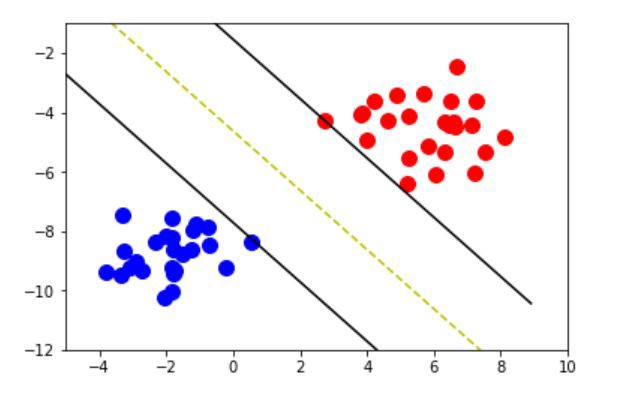
\includegraphics[width=14cm]{images/svm.jpeg}
			\end{figure} \\
			\hline
		\end{tabular}
	\end{adjustbox}
	\captionof{figure}{Contoh \textit{Hyperplane} pada SVM}
	\label{fig:hyperplanesvm}
\end{table}

\noindent SVM pada mulanya digunakan untuk menangani klasifikasi yang terdiri dari 2 kelas saja. Namun seriring dengan perkembangan zaman masalah yang dihadapi semakin kompleks sehingga membutuhkan teknik untuk melakukan proses klasifikasi lebih dari 2 kelas. Untuk melakukan klasifikasi lebih dari 2 kelas, terdapat 2 pendekatan yang bisa digunakan yaitu \textit{One-Versus-One} dan \textit{One-Versus-Rest}. Pada pendekatan \textit{One-Versus-One}, akan dibuat sebanyak $k(k-1)/2$  pasangan kelas untuk pengujian untuk klasifikasi dengan kelas sebanyak $k$. Untuk menentukan kelas mana yang menjadi klasifikasi untuk suatu kumpulan data caranya adalah sistem \textit{voting}. Kelas dengan jumlah \textit{voting} terbanyak akan menjadi \textit{classifier} untuk data tersebut. Pada pendekatan \textit{One-Versus-Rest} akan dibuat sebanyak $k$ pasangan kelas untuk klasifikasi dengan kelas sebanyak $k$. Setiap kelas yang diuji akan dibandingkan dengan sisa kelas yang ada. Misal terdapat 3 kelas A,B, dan C, maka kelas A akan dibandingkan dengan kelas B dan C, kelas B dibandingkan dengan kelas A dan C, kelas C dibandingkan dengan kelas A dan B. Kekurangan dari pendekatan ini adalah jumlah \textit{training set} yang tidak seimbang \cite{svm}.

\noindent Untuk proses klasifikasi \textit{non-linear} dapat dicari dengan persamaan 2.13 berikut:
\begin{table}[H]
	\small
	\begin{adjustbox}{width=1\textwidth}
		\begin{tabular}{|p{13.55cm}|}
			\hline
			\begin{equation}
			f(x) = sign(\sum_{i=1}^{l}\alpha_iy_iK(x,x_i)+b)
			\end{equation}\\
			\hline
		\end{tabular}
	\end{adjustbox}
\end{table}
\noindent
\renewcommand{\arraystretch}{1} 
\begin{tabularx}{\textwidth}{lll}
	Dimana: \\
	$l$ & = & Banyaknya kelas citra\\
	$\alpha_i$ & = & Nilai alpha ke $i$\\
	$y_i$ & = & Nilai kelas citra ke $i$\\
	$K(x,x_i)$ & = & Fungsi kernel\\
	$b$ & = & Nilai bias\\
\end{tabularx}

\noindent Nilai $\alpha$ dan $b$ dapat dicari dengan persamaan linear yang membentuk \textit{hyperplane} SVM. Persamaan \ref{eq:PersamaanSVM1} sampai \ref{eq:PersamaanSVM2} berikut merupakan persamaan \textit{hyperplane} SVM:

\begin{table}[H]
	\small
	\begin{adjustbox}{width=1\textwidth}
		\begin{tabular}{|p{13.55cm}|}
			\hline
			\begin{equation}
			\sum_{i=1}^{l}\alpha_iy_iK(x,x_i)+b)=0
			\label{eq:PersamaanSVM1}
			\end{equation}
			\begin{equation}
			\sum_{i=1}^{l}\alpha_iy_iK(x,x_i)+b)=1
			\end{equation}
			\begin{equation}
			\sum_{i=1}^{l}\alpha_iy_iK(x,x_i)+b)=-1
			\label{eq:PersamaanSVM2}
			\end{equation}\\
			\hline
		\end{tabular}
	\end{adjustbox}
\end{table}
\noindent
\renewcommand{\arraystretch}{1} 
\begin{tabularx}{\textwidth}{lll}
	Dimana: \\
	$l$ & = & banyaknya kelas citra\\
	$\alpha_i$ & = & nilai alpha ke $i$\\
	$y_i$ & = & nilai kelas citra ke $i$\\
	$K(x,x_i)$ & = & fungsi kernel\\
	$b$ & = & nilai bias\\
\end{tabularx}

\noindent Seringkali kasus yang ada dalam dunia nyata tidak selalu bisa dipisahkan secara linier (\textit{linearly separable}) seperti pada contoh gambar di atas. Misalnya suatu kumpulan data memiliki fitur yang memiliki n-dimensi. Linear SVM tidak bisa diterapkan untuk kasus tersebut, sehingga diperlukan teknik agar membuat \textit{hyperplane} yang bisa memisahkan antara 2 kelas dalam ruang multidimensi. Cara yang umum digunakan untuk menyelesaikan masalah tersebut adalah dengan menggunakan kernel. Kernel yang umum digunakan pada SVM yaitu \textit{Radial Basis Function} seperti pada persamaan \ref{eq:PersamaanRBF} berikut:

\begin{table}[H]
	\small
	\begin{adjustbox}{width=1\textwidth}
		\begin{tabular}{|p{13.55cm}|}
			\hline
			\begin{equation}
			RBF = K(x_i,x_j) = \exp (-\frac{\|x_i-x_j\|}{2\sigma^2})
			\label{eq:PersamaanRBF}
			\end{equation}\\
			\hline
		\end{tabular}
	\end{adjustbox}
\end{table}
\noindent
\renewcommand{\arraystretch}{1} 
\begin{tabularx}{\textwidth}{lll}
	Dimana: \\
	$K$ & = & nilai fungsi kernel RBF\\
	$x_i$ & = & vektor input 1\\
	$x_j$ & = & vektor input 2\\
	$\sigma$ & = & konstanta sigma\\
\end{tabularx}
\vspace{4.5pt}

\subsection{\textit{Confusion Matrix}}
\noindent \textit{Confusion Matrix} merupakan metode pengukuran untuk mengevaluasi hasil klasifikasi. Dengan melakukan klasifikasi sebanyak $C$ kelas, dihasilkan \textit{confusion matrix} $M$ berukuran $C \times C$, di mana elemen $M_{ij}$ dalam matriks menunjukkan jumlah sampel yang salah diklasifikasikan, sementara $M_{ii}$ adalah jumlah sampel yang hasil klasifikasinya adalah benar. \textit{Confusion matrix} pada gambar \ref{fig:ConfusionMatrix} digunakan pada kasus klasifikasi dua buah kelas sehingga membentuk matriks berukuran $2 \times 2$ \cite{markham}.

\begin{adjustbox}{width=1\textwidth}
\noindent\begin{minipage}{\linewidth}
	\framebox[\textwidth]{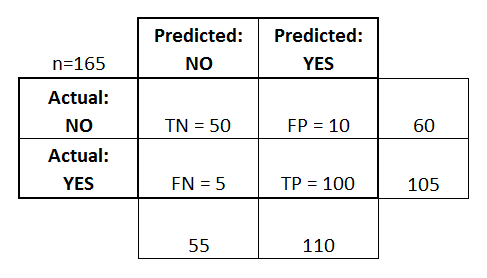
\includegraphics[width=8cm]{images/ConfusionMatrixForBinaryClassification.png}}
	\captionof{figure}{\textit{Confusion Matrix untuk Dua Kelas} \cite{markham}}
	\label{fig:ConfusionMatrix}
\end{minipage}
\end{adjustbox}

\noindent Elemen $M_{11}$ pada matriks menunjukkan jumlah sampel yang pada kenyataannya adalah kelas 1 dan diklasifikasikan sebagai kelas 1, sehingga disebut sampel \textit{true-positive} (TP). Elemen $M_{12}$ menunjukkan jumlah sampel yang pada kenyataannya adalah kelas 1 tetapi diklasifikasikan sebagai kelas -1, sehingga disebut sampel \textit{false-negative} (FN). Elemen $M_{21}$ menunjukkan jumlah sample yang pada kenyataannya adalah kelas -1 tetapi diklasifikasikan sebagai kelas 1, sehingga disebut sampel \textit{false-positive} (FP). Dan elemen $M_{22}$ menunjukkan jumlah sampel yang kenyataannya adalah kelas -1 dan diklasifikasikan sebagai kelas -1, sehingga disebut \textit{true-negative} (TN). Maka untuk menghitung akurasi dapat digunakan persamaan \ref{eq:accuracy}. Hasil akurasi yang semakin baik akan mendekati nilai 1, sebaliknya akurasi yang buruk mendekati nilai 0.
\begin{table}[H]
	\begin{adjustbox}{width=1\textwidth}
	\begin{tabular}{|p{13.55cm}|}
		\hline
		\begin{equation}
			Accuracy = \frac{TP + TN}{TP + TN + FP + FN}
			\label{eq:accuracy}
		\end{equation}\\
	\hline
	\end{tabular}
	\end{adjustbox}
\end{table}

Lalu perhitungan \textit{precision} yang merupakan perbandingan dari hasil positif dapat dihitung dengan persamaan \ref{eq:precision}.
\begin{table}[H]
	\begin{adjustbox}{width=1\textwidth}
	\begin{tabular}{|p{13.55cm}|}
		\hline
		\begin{equation}
			Precision = \frac{TP}{TP + FP}
			\label{eq:precision}
		\end{equation}\\
	\hline
	\end{tabular}
	\end{adjustbox}
\end{table}

Dan perhitungan \textit{recall} atau disebut juga sebagai sensitivitas dapat dihitung dengan persamaan \ref{eq:recall}.
\begin{table}[H]
	\begin{adjustbox}{width=1\textwidth}
	\begin{tabular}{|p{13.55cm}|}
		\hline
		\begin{equation}
			Recall = \frac{TP}{TP + FN}
			\label{eq:recall}
		\end{equation}\\
	\hline
	\end{tabular}
	\end{adjustbox}
\end{table}

\subsection{Penggunaan \textit{Library}}
\noindent Berikut adalah penjelasan dari \textit{library} yang digunakan di dalam penelitian. \\
\subsubsection{OpenCV}
\noindent\textit{Library} yang digunakan adalah OpenCV untuk proses \textit{pre-processing} citra. OpenCV merupakan \textit{library open-source} yang banyak digunakan untuk penelitian terkait proses pengolahan citra dan \textit{computer vision}. 
\begin{small}
	\begin{longtable}{| p {0.5cm} | p {6cm} | p {6cm} |}
		\caption{Tabel fungsi \textit{Library} OpenCV} \\
		\hline
		\textbf{No}  & \textbf{\textit{Function}}  & \textbf{Deskripsi} \\
		\hline
		\endfirsthead
		\endhead
		1 & Imgcodecs.imread(String filename) & Mengambil citra dari \textit{path} yang diisikan ke parameter.\\
		\hline
		2 & Imgproc.cvtColor(Mat src, Mat dst, int code) & Mengubah jenis warna pada citra sesuai yang diinginkan. Parameter fungsi ini terdiri dari Mat asal, Mat tujuan, dan \textit{code}. \textit{Code} digunakan untuk memilih tipe konversi citra tersebut, misal \textit{grayscale}.\\
		\hline
		3 & Imgproc.Canny(Mat image,Mat edges,double threshold1, double threshold2) & Fungsi ini digunakan untuk mendeteksi tepian pada citra menggunakan Canny.\\
		\hline
	\end{longtable}
\end{small}
\subsubsection{Weka}
\noindent Weka adalah kumpulan dari algoritme pembelajaran mesin yang digunakan untuk menyelesaikan permasalahan \textit{data mining}. \textit{Library} ini berbasis bahasa pemrograman Java dan dapat berjalan di hampir seluruh platform. Dalam penelitian ini, \textit{library} Weka digunakan untuk melakukan proses klasifikasi menggunakan metode \textit{Support Vector Machine}.
\begin{small}
	\begin{longtable}{| p {0.5cm} | p {6cm} | p {6cm} |}
		\caption{Tabel fungsi \textit{Library} Weka} \\
		\hline
		\textbf{No}  & \textbf{\textit{Function}}  & \textbf{Deskripsi} \\
		\hline
		\endfirsthead
		\endhead
		1 & libsvm.setOptions(String options) & Mengkonfigurasi \textit{classifier} yang akan digunakan.\\
		\hline
		2 & libsvm.buildClassifier(Instances insts) & Membangun \textit{classifier} sesuai dengan konfigurasi yang digunakan dan dataset yang diberikan.\\
		\hline
	\end{longtable}
\end{small}

\section{Tinjauan Studi}
\noindent Pada bagian ini akan dijelaskan mengenai perbandingan dari berbagai penelitian terkait metode deteksi dan pengenalan plat nomor mobil. \\

\subsection{\textit{State of the Art}}
\noindent Terdapat beberapa metode lain yang memiliki ruang lingkup yang mirip dengan penelitian ini khususnya mengenai deteksi dan pengenalan plat nomor mobil. Tabel \ref{tbl:StateoftheArt} \textit{State of the Art} akan menjelaskan perbedaan-perbedaan metode dari jurnal terkait.\\
\\
\\
\\
\\
\\
\\
\\
\\
\begingroup
\setlength{\LTleft}{-20cm plus -1fill}
\setlength{\LTright}{\LTleft}
\begin{small}
\begin{longtable}{ |p{5cm}|p{3.5cm}|p{3.6cm}| }
\caption{\textit{State of the Art}}\\
\hline
\textbf{Jurnal} & \textbf{Rumusan Masalah} & \textbf{Metode}\\
\endfirsthead

\multicolumn{3}{c}{\textbf{\tablename~\thetable} \textit{State of the Art} (Lanjutan)}\\
\hline
\textbf{Jurnal} & \textbf{Rumusan Masalah} & \textbf{Metode}\\
\endhead

\hline
 Gou, C., Wang, K., Yao, Y., Li, Z. (2016). Vehicle license plate recognition based on extremal regions and restricted Boltzmann machines. \emph{IEEE Transactions on Intelligent Transportation Systems, 17}(4), 1096-1107. & Apakah dengan menerapkan pendeteksian plat nomor dengan \textit{Extremal Region} dan pengenalan karakter plat nomor menggunakan \textit{Hybrid Discriminative Restricted Boltzmann Machine} dapat meningkatkan akurasi pendeteksian dan pengenalan dalam berbagai kondisi cuaca dan \textit{background} yang kompleks? & 
\begin{enumerate}[wide, labelwidth=!, labelindent=0pt, topsep=0pt]
\item \textit{Extremal Region}
\item \textit{AdaBoost}
\item \textit{Histogram of Oriented Gradient}
\item \textit{Hybrid Discriminative Restricted Boltzmann Machine} 
\end{enumerate}\\
\hline
 Gou, C., Wang, K., Yu, Z., Xie, H. (2014, October). License plate recognition using MSER and HOG based on ELM. In \emph{Proceedings of 2014 IEEE International Conference on Service Operations and Logistics, and Informatics} (pp. 217-221). IEEE. & Apakah dengan menerapkan \textit{Maximally Stable Extremal Region} untuk pendeteksian plat nomor dan \textit{Extreme Learning Machine} untuk pengenalan karakter plat nomor dapat meningkatkan performa dan akurasi sistem? & 
\begin{enumerate}[wide, labelwidth=!, labelindent=0pt, topsep=0pt]
\item \textit{Maximally Stable Extremal Region}
\item \textit{Histogram of Oriented Gradient}
\item \textit{Extreme Learning Machine}
\end{enumerate}\\
\hline
Tabrizi, S. S., Cavus, N. (2016). A hybrid KNN-SVM model for Iranian license plate recognition. \emph{Procedia Computer Science, 102}, pp. 588-594. & Apakah dengan menggabungkan metode klasifikasi \textit{K-Nearest Neighbours} dan \textit{Support Vector Machine} akan menghasilkan akurasi yang lebih baik dan mengurangi \textit{cost} pada proses pengenalan karakter plat nomor kendaraan? &
\begin{enumerate}[wide, labelwidth=!, labelindent=0pt, topsep=0pt]
\item \textit{Structural Feature}
\item \textit{Horizontal and Vertical Crossing Count Histogram}
\item \textit{Zoning Feature Extraction}
\item \textit{K-Nearest Neigbhours}
\item \textit{Support Vector Machine}
\end{enumerate}\\
\hline
Rasheed, S., Naeem, A., Ishaq, O. (2012, October). Automated number plate recognition using hough lines and template matching. In \emph{Proceedings of the World Congress on Engineering and Computer Science} (Vol. 1, pp. 24-26). & Apakah dengan menggunakan metode \textit{Hough Transform} untuk mendeteksi plat kendaraan dan \textit{Template Matching} untuk pengenalan karakter dapat menghasilkan akurasi yang baik untuk sistem pengenalan plat nomor kendaraan? &
\begin{enumerate}[wide, labelwidth=!, labelindent=0pt, topsep=0pt]
	\item \textit{Canny Detector}
	\item \textit{Hough Transform}
	\item \textit{Morphological Process}
	\item \textit{Template Matching}
\end{enumerate}\\
\hline
Nugroho, A., Wardhani, K.R.R. (2011). Aplikasi Sistem Pembaca Plat Nomor Mobil Menggunakan Pengolahan Citra dan Metode Learning Vector Quantization. & Apakah dengan menerapkan pengolahan citra untuk deteksi plat kendaraan dan metode \textit{Learning Vector Quantization} untuk pengenalan karakter dapat menghasilkan akurasi yang baik ? &
\begin{enumerate}[wide, labelwidth=!, labelindent=0pt, topsep=0pt]
	\item \textit{Pengolahan Citra}
	\item \textit{Learning Vector Machine}
\end{enumerate}
\label{tbl:StateoftheArt}\\
\hline
\end{longtable}
\end{small}
\endgroup
 
\subsection{Pembahasan Penelitian Terkait}
\noindent Terdapat beberapa metode yang dapat khususnya untuk mendeteksi plat nomor dan mengenali karakter pada plat nomor.
\noindent Pada referensi pertama \cite{gou2016} menggunakan metode \textit{Extremal Region} sebagai proses untuk mendapatkan daerah-daerah karakter dari suatu plat nomor, kemudian \textit{Extremal Region} yang didapat diseleksi dengan menggunakan \textit{AdaBoost} sehingga bisa didapatkan daerah karakter plat nomor yang sesuai dengan kriteria yang diinginkan, dari daerah-daerah karakter yang didapatkan barulah kandidat plat nomor yang benar bisa didapatkan. Proses selanjutnya adalah pengambilan fitur karakter dengan menggunakan metode \textit{Histogram of Oriented Gradient} sehingga didapatkan fitur vektor dari setiap karakter pada plat nomor, yang nantinya akan menjadi masukkan bagi metode klasifikasi \textit{Hybrid Discriminative Restricted Boltzmann Machine}.

\noindent Pada referensi kedua \cite{gou2014} menggunakan metode \textit{Maximally Stable Extremal Region} untuk memilih kandidat daerah karakter yang nantinya akan menentukan lokasi dari plat nomor berdasarkan letak geometris dari kandidat-kandidat karakter tersebut. Setelah lokasi plat nomor didapatkan, \textit{HOG Descriptor} dari setiap karakter diambil dengan menggunakan metode \textit{Histogram of Oriented Gradient} dan setiap karakternya akan dikenali menggunakan metode \textit{neural network} bernama \textit{Extreme Learning Machine}.

\noindent Pada referensi ketiga \cite{tabrizi} digabungkan metode klasifikasi \textit{K-Nearest Neighbours} dengan metode klasifikasi \textit{Support Vector Machine}. \textit{K-Nearest Neighbours} digunakan karena sifatnya yang mudah dipelajari, bersifat tangguh terhadap data yang memiliki derau dan efektif jika jumlah yang dimiliki berjumlah banyak. Sedangkan metode \textit{Support Vector Machine} digunakan untuk karakter-karakter yang memiliki kemiripan karakteristik, sehingga akurasi dari pengenalan karakter dapat meningkat.

\noindent Pada referensi keempat \cite{rasheed} menggunakan \textit{Hough Transform} untuk mendeteksi lokasi plat kendaraan dan menghasilkan akurasi yang baik, yaitu sekitar 94\% untuk plat nomor yang terdeteksi dan dengan menggunakan metode \textit{Template Matching} menghasilkan akurasi pengenalan karakter plat nomor kendaraan sebesar 90\%.

\noindent Pada referensi kelima \cite{nugroho} menggunakan metode pengolahan citra untuk mencari kandidat-kandidat pita dengan menghitung grafik vertikal gambar untuk mendapatkan lokasi plat nomor kendaraan, kemudian setiap karakter dari plat nomor yang didapatkan disegmentasi dengan cara menghitung grafik horizontal gambar, kemudian untuk metode klasifikasi karakter yang digunakan adalah \textit{Learning Vector Quantization}.\\

\section{Tinjauan Objek}
\noindent Pada bagian ini akan diulas mengenai objek-objek yang terkait dengan deteksi dan pengenalan plat nomor kendaraan.\\

\subsection{Tanda Nomor Kendaraan Bermotor}
\noindent Tanda Nomor Kendaraan Bermotor (disingkat TNKB) disebut juga sebagai plat nomor atau nomor polisi adalah plat aluminium tanda kendaraan bermotor di Indonesia yang telah didaftarkan pada Kantor Bersama Samsat.

\begin{adjustbox}{width=1\textwidth}
\noindent\begin{minipage}{\linewidth}
	\centering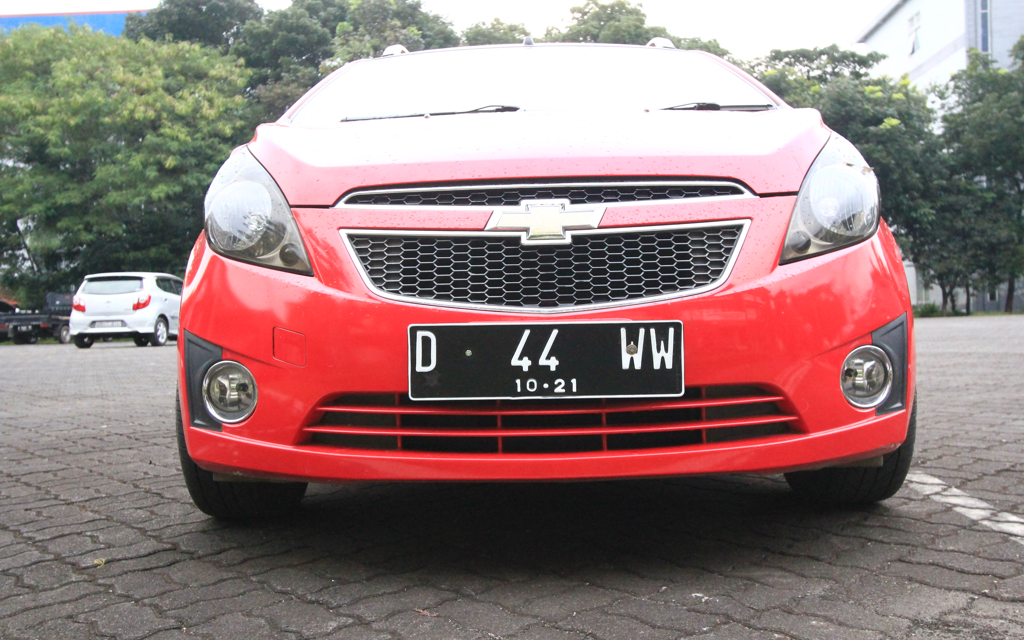
\includegraphics[width=12cm]{images/plat_nomor_example.png}
	\captionof{figure}{Contoh dari plat nomor kendaraan Indonesia}
	\label{fig:ContohPlatNomorIndonesia}
\end{minipage}
\end{adjustbox}\\

\subsection{Spesifikasi Teknis}
\noindent Plat nomor kendaraan Indonesia terdiri dari cetakan tulisan dua baris, pada baris pertama terdapat tiga hal yang diinformasikan, yaitu kode wilayah(huruf), nomor polisi(angka), dan kode/seri akhir wilayah(huruf). Sedangkan baris kedua menunjukkan bulan dan tahun masa berlaku, masing-masing dua digit. Contohnya pada gambar \ref{fig:ContohPlatNomorIndonesia} angka yang terdapat di baris keduanya adalah 10.21. Hal tersebut menandakan bahwa plat nomor tersebut akan habis masa berlakunya pada bulan Oktober tahun 2021.

\noindent Bahan baku dari plat nomor adalah aluminium dengan ketebalan 1mm. Ukuran plat nomor untuk kendaraan bermotor roda dua dan roda tiga adalah 250 $\times$ 105 mm, sedangkan untuk kendaraan bermotor roda empat atau lebih adalah 395 $\times$ 135 mm. Terdapat cetakan garis lurus pembatas selebar 5mm di antara ruang nomor polisi dengan ruang angka masa berlaku (untuk plat nomor lama), sedangkan semenjak tahun 2011 di sekitar plat nomor terdapat garis putih dan tidak ada garis pemisah antara nomor polisi dan masa berlaku.

\noindent Pada tahun 2014 terjadi perubahan tampilan pada plat nomor untuk kendaraan bermotor roda empat. Plat nomor kini sedikit lebih panjang dari sebelumnya (5 cm lebih panjang) untuk memberi ruang pada kode/seri akhir wilayah yang dulunya berjumlah dua digit menjadi tiga digit.\\

\subsection{Jenis TNKB}
\noindent Jenis dari TNKB di Indonesia dibedakan berdasarkan warna dari TNKB tersebut, warna TNKB yang ditetapkan di Indonesia adalah sebagai berikut:
\begin{enumerate}
\item Kendaraan pribadi dan sewa: warna dasar hitam dengan tulisan berwarna putih.
\item Kendaraan umum: warna dasar kuning dengan tulisan hitam.
\item Kendaraan milik pemerintah: warna dasar merah dengan tulisan berwarna putih.
\item Kendaraan bermotor sementara: warna dasar putih dengan tulisan berwarna merah.
\item Kendaraan korps diplomatik negara asing: warna dasar putih/merah dengan tulisan berwarna hitam.
\item Kendaraan staf operasional korps diplomatik negara asing: warna dasar hitam dengan tulisan berwarna putih serta terdiri dari lima angka dan kode angka negara yang dicetak lebih kecil dengan format sub-bagian.
\end{enumerate}

%\subsubsection{Pendeteksian dan Pelacakan Manusia}
%\noindent Pada bagian ini akan dijelaskan beberapa teori mengenai deteksi manusia dan pelacakan manusia.\\

%\subsubsection{Deteksi dan Melacak Manusia}
%\noindent Pendeteksian manusia adalah proses atau tahap awal untuk menemukan dan menentukan posisi objek manusia dari sebuah citra. Pendeteksian manusia ini fokus untuk menemukan bagian atas badan manusia dari tampak depan maupun tampak belakang, seperti yang terlihat pada gambar \ref{fig:ContohDeteksiManusia}. Sementara pelacakan manusia adalah proses untuk mengikuti jejak pergerakan dari objek manusia yang telah terdeteksi pada tahap sebelumnya. Tahap ini menggunakan estimasi perubahan atau pergerakan sehingga tidak perlu terus-menerus melakukan proses pendeteksian manusia pada setiap citra.\\
%\begin{adjustbox}{width=1\textwidth}
%\noindent\begin{minipage}{\linewidth}
%	\framebox[\textwidth]{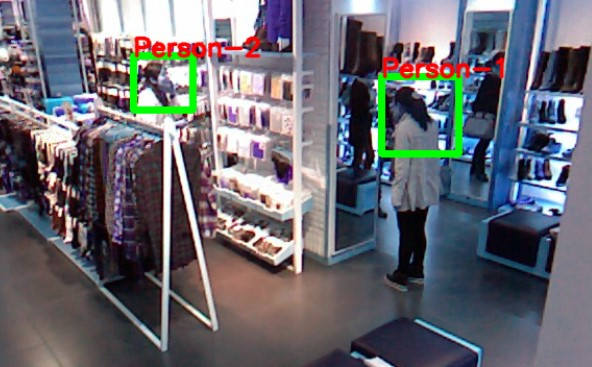
\includegraphics[width=8cm]{images/DeteksiManusia.jpg}}
%	\captionof{figure}{Contoh dari pendeteksian manusia \cite{15}}
%	\label{fig:ContohDeteksiManusia}
%\end{minipage}
%\end{adjustbox}\\

%\subsection{\textit{Database RGB-D}}
%\noindent \textit{Database RGB-D} didapatkan dari \textit{Fudan University}. \textit{Fudan University} memiliki dan menyediakan \textit{database} yang dapat digunakan secara gratis oleh umum. Dalam penelitian ini digunakan 2 buah \textit{dataset} positif yang terdapat manusia di dalamnya, ditangkap oleh \textit{Fudan University} menggunakan sensor Microsoft Kinect yang memiliki resolusi berukuran 640 $\times$ 480 dengan \textit{frame rate} 30 fps. Sensor yang digunakan Microsoft Kinect dapat menangkap sepasang citra dalam waktu bersamaan yaitu citra RGB dan citra kedalaman sehingga menjadi citra RGB-D.

%\noindent Dalam masing-masing \textit{dataset} terdapat sepasang kumpulan citra yaitu citra tipe RGB dan citra kedalaman. Selain itu, diberitahukan juga koordinat \textit{ground truth} pada setiap pasangan citra yang menandakan posisi manusia yang terdapat pada citra tersebut.
%\textit{Dataset} yang pertama bernama \textit{Clothing Store RGBD}, berada pada salah satu toko pakaian dengan jumlah citra 1.000 buah untuk masing-masing tipe citra. Dalam 1.000 citra tersebut terdapat 2.367 posisi manusia pada berkas \textit{ground truth}. Contoh sepasang citra yang terdapat pada \textit{dataset} pertama dapat dilihat pada gambar \ref{fig:DatasetClothingStore}, di mana seharusnya terdapat 2 orang yang terdeteksi. \\
%\begin{adjustbox}{width=1\textwidth}
%\noindent\begin{minipage}{\linewidth}
%	\framebox[\textwidth]{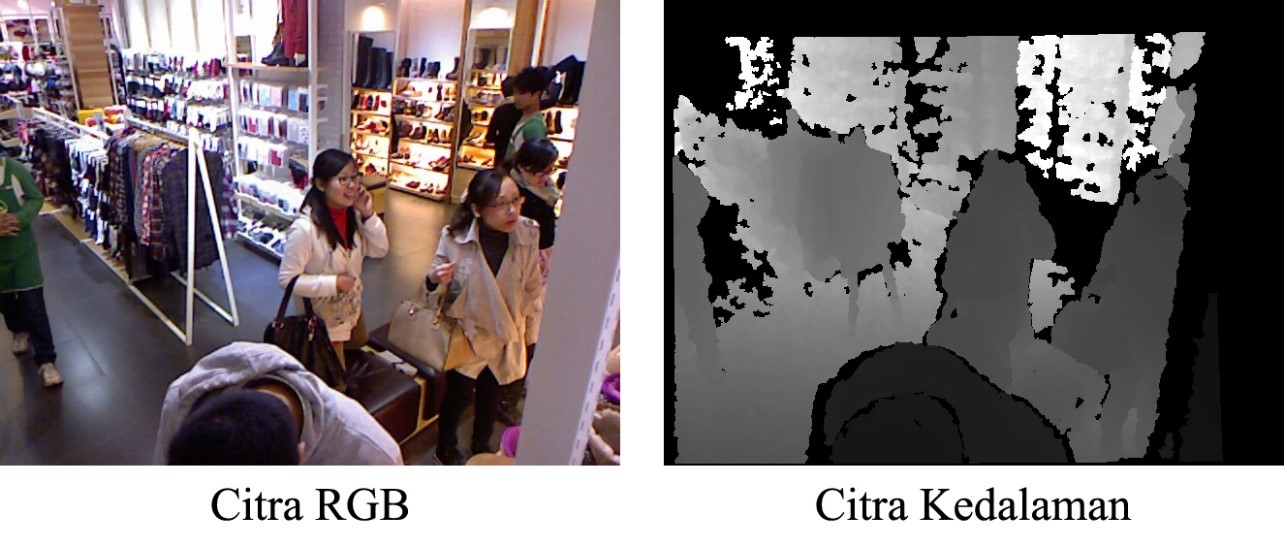
\includegraphics[width=12cm]{images/DBClothingStore.jpg}}
%	\captionof{figure}{\textit{Dataset} CLOTHING STORE \cite{15}}
%	\label{fig:DatasetClothingStore}
%\end{minipage}
%\end{adjustbox}\\

%\noindent Pada gambar \ref{fig:GroundTruthClothingStore} terlihat \textit{ground truth} dari setiap citra \textit{dataset Clothing Store}, di mana angka awal sebelum titik dua merupakan citra pada waktu \textit{fps} tertentu dan setiap kurung siku menyatakan keberadaan posisi manusia pada citra, yang masing-masing terdiri atas $x_{1},y_{1}$ untuk koordinat titik kiri atas dan $x_{2},y_{2}$ untuk koordinat titik kanan bawah. \\
%\begin{adjustbox}{width=1\textwidth}
%\noindent\begin{minipage}{\linewidth}
%	\framebox[\textwidth]{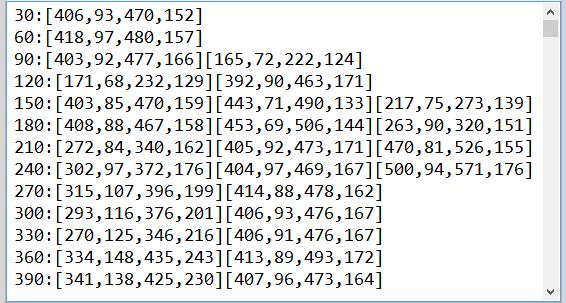
\includegraphics[width=8cm]{images/GroundTruthClothingStore.jpg}}
%	\captionof{figure}{Berkas \textit{ground truth} CLOTHING STORE \cite{15}}
%	\label{fig:GroundTruthClothingStore}
%\end{minipage}
%\end{adjustbox}\\

%\noindent Untuk dataset kedua bernama \textit{Outdoor crowds in the dark RGBD}, berada di lingkungan \textit{Fudan University} pada malam hari sehingga kondisi pencahayaannya relatif redup dengan jumlah citra total adalah 275 buah untuk masing-masing tipe citra. Berbeda dengan \textit{dataset} pertama, pada \textit{dataset Outdoor} terdapat tiga buah folder bernama 31, 54, dan 56. Jumlah citra pada masing-masing folder bervariasi dan telah dilengkapi dengan berkas \textit{ground truth}. Penjelasan lebih rinci mengenai \textit{dataset} ini dapat dilihat pada tabel \ref{tbl:Outdoor}.
%\begin{table}[H]
%\centering
%\begin{small}
%\captionof{table}{Rincian \textit{Dataset Outdoor} \label{tbl:Outdoor}}
%\begin{tabular}{|p{1cm}|p{3cm}|p{3cm}|}
%	\hline
%	\textbf{Folder} & \textbf{Jumlah Citra} & \textbf{Jumlah Posisi Manusia}\\
%	\hline
%	31 & 57 & 273 \\
%	\hline
%	54 & 95 & 427 \\
%	\hline
%	56 & 123 & 548 \\
%	\hline
%\end{tabular}
%\end{small}
%\end{table}

%\noindent Contoh sepasang citra yang terdapat pada dataset kedua dapat dilihat pada gambar \ref{fig:DatasetOutdoor}, di mana seharusnya terdapat 6 orang yang terdeteksi. \\
%\begin{adjustbox}{width=1\textwidth}
%\noindent\begin{minipage}{\linewidth}
%	\framebox[\textwidth]{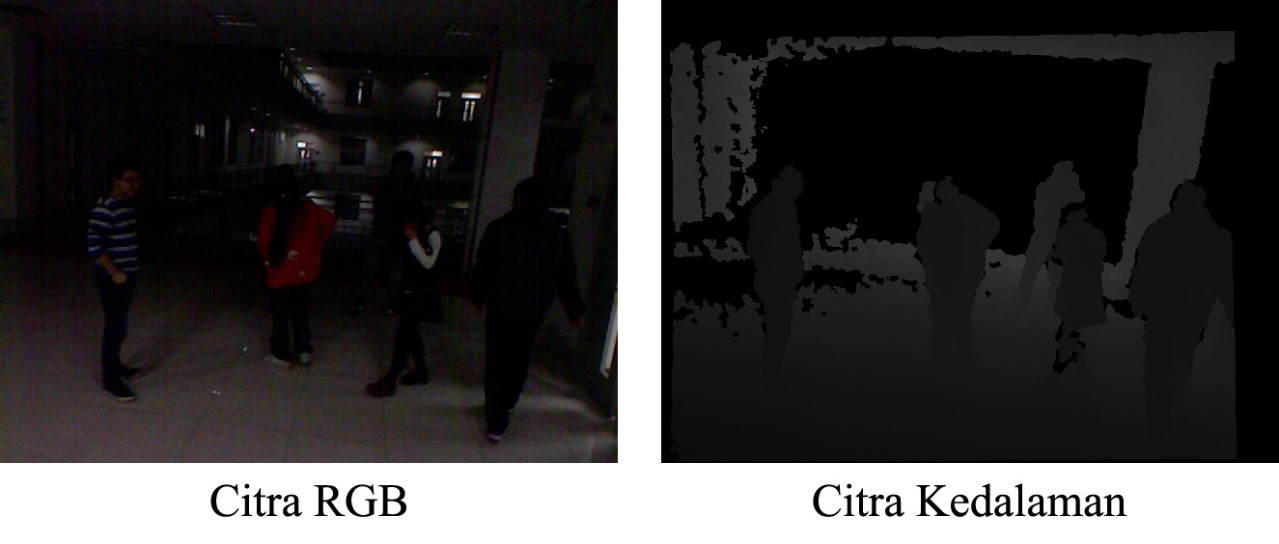
\includegraphics[width=12cm]{images/DBOutdoor.jpg}}
%	\captionof{figure}{\textit{Dataset} OUTDOOR \cite{15}}
%	\label{fig:DatasetOutdoor}
%\end{minipage}
%\end{adjustbox}\\

%\noindent Pada gambar \ref{fig:GroundTruthOutdoor} terlihat \textit{ground truth} dari setiap citra \textit{dataset Outdoor}, di mana nilai yang berada dalam tanda kutip dua merupakan lokasi dengan nama citra dan setiap nilai di dalam tanda kurung menyatakan keberadaan posisi manusia pada citra, yang masing-masing terdiri atas $x_{1},y_{1}$ untuk koordinat titik kiri atas dan $x_{2},y_{2}$ untuk koordinat titik kanan bawah. \\
%\begin{adjustbox}{width=1\textwidth}
%\noindent\begin{minipage}{\linewidth}
%	\framebox[\textwidth]{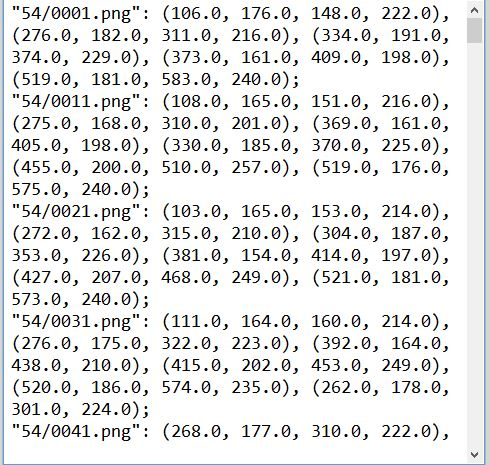
\includegraphics[width=8cm]{images/GroundTruthOutdoor.jpg}}
%	\captionof{figure}{Berkas \textit{ground truth} OUTDOOR \cite{15}}
%	\label{fig:GroundTruthOutdoor}
%\end{minipage}
%\end{adjustbox}\\

%\noindent \textit{Dataset} pertama akan dibagi dengan perbandingan 80:20, 80\% akan digunakan sebagai \textit{data training} dan 20\% digunakan sebagai {data testing}. Untuk \textit{dataset} kedua, folder 56 akan digunakan sebagai \textit{data training} dan folder 31 dan 54 digunakan sebagai {data testing}. \textit{Dataset} negatif yang tidak mengandung manusia akan diambil secara acak berukuran 65 $\times$ 80 dari masing-masing \textit{dataset} dengan ketentuan, tidak berpotongan dengan posisi \textit{ground truth}.

\newpage